\section{W02 - OP Strategy \& Performance}
 
\subsection{Role of Operations}
\subsubsection{The Strategic Role of Operations can be defined by its aspirations (Hayes and Wheelwright)}
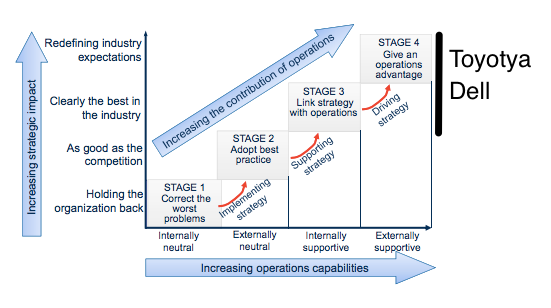
\includegraphics[width=1\textwidth]{W02/role_of_operations}
\textbf{STAGE 2 Best Practise}\\ so gut wie die anderen, nach heutigem standard. Kunde nimt einen als normalen Anbieter wahr\\
\textbf{STAGE 3: Best in Class}\\ Vorsprung wie kurze Lieferzeiten oder Preis. Kunde merkt das noch nicht.\\
\textbf{STAGE 4}\\ Nur 1 mal in der Branche. \textbf{Kunde} bemerkt Anbieter und \textbf{kommt selbst\"andig}
\index{Best in Class}
\index{Best Practice}
\index{Hayes}
\index{Wheelwright}
\subsubsection{Broad Strategic Objectives for an Operation Applied to Stakeholder Groups}
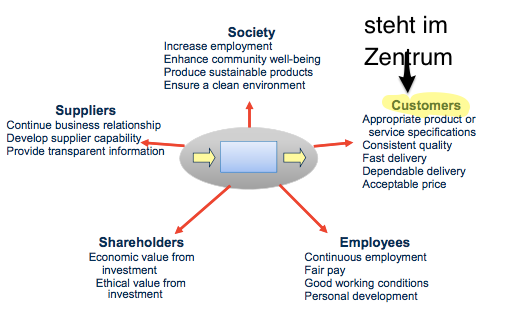
\includegraphics[width=1\textwidth]{W02/stakeholder_group}
\index{Stakeholder!Groups}
\index{Operation!Objectives}
\subsection{Operations Goals}
\subsubsection{The Five Performance Goals\index{Five Performance Goals}}\label{FivePerformanceGoals}
\index{5!Leistungsziele}
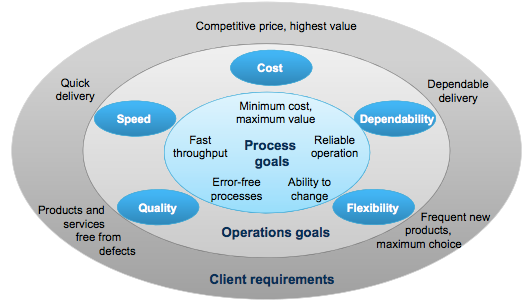
\includegraphics[width=1\textwidth]{W02/5_performance_goals}
\subsubsection{Performance Goals\index{Performance Goals} and \index{Competitive Factors}Competitive Factors}
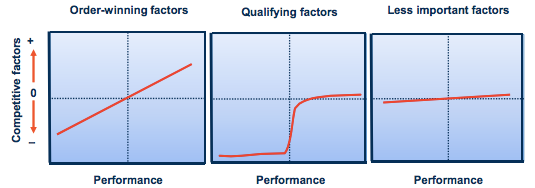
\includegraphics[width=1\textwidth]{W02/performancegoals}
\index{Factor!Order-Winning}Order-winnning factors: bei kleinen Performancever\"anderungen grosser ''Gewinn''\\
\index{Factor!Qualifying}Qualifying factors: wenn minimum nicht erreicht wird, Kunde/Auftrag verloren
\subsubsection{The Five Competitive Objectives}
\index{Competitive Objectives}
\begin{tabular}{rl}
Quality &  RIGHT\\
Speed &  FAST\\
Dependability & ON TIME\\
Flexibility & ABLE TO CHANGE\\
Cost & PRODUCTIVE\\
\end{tabular} 
= Competitivenesse\index{Competitivenesse}
\subsubsection{The Effects of the Product/Service Life Cycle on an Operation’s Performance Objectives}
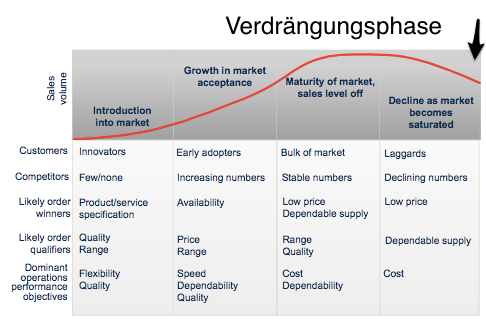
\includegraphics[width=1\textwidth]{W02/productlifecycle}
\subsubsection{Quality Means Different Things in Different Operations}
\begin{center}
\begin{tabular}{|c|c|}
	\hline Hospital & Automobile plant \\ 
	\hline Bus company & Supermarket \\ 
	\hline 
\end{tabular} 
\end{center}
\subsubsection{Cost Means Different Things in Different Operations}
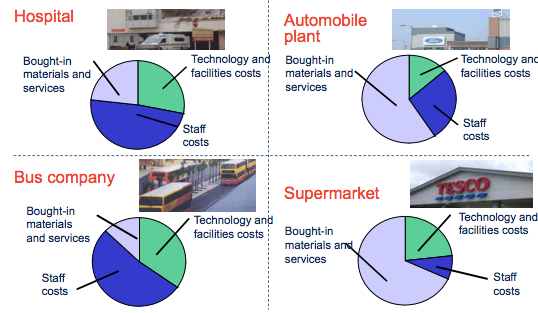
\includegraphics[width=1\textwidth]{W02/cost_operations}
\subsubsection{Polar Diagrams}
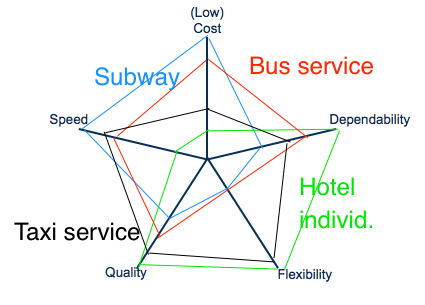
\includegraphics[width=1\textwidth]{W02/polar_diagramm}
\subsection{Strategy and Trade-Offs}
\subsubsection{What is Strategy? }\label{whatIsStrategy}
Das Kriegsche Modell\index{Kriegsche Modell}:\\
Values are fix, and mid-term goals are reacting on values.\\
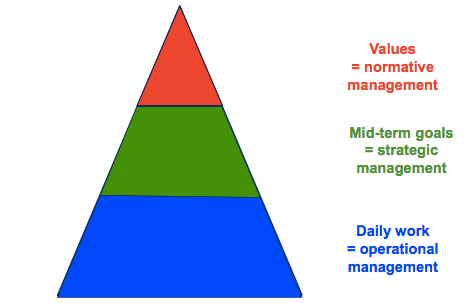
\includegraphics[width=1\textwidth]{W02/strategy}
\subsubsection{Operational Management Executes the Operations Strategy}
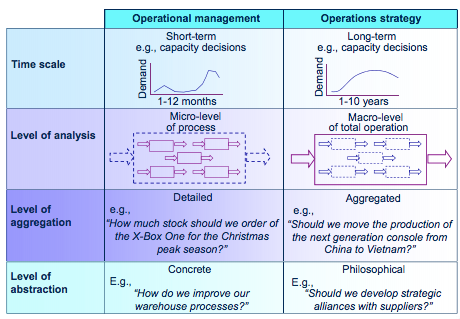
\includegraphics[width=1\textwidth]{W02/operations_strategy}
\index{Operational!Management}
\index{Operational!Strategy}
\subsubsection{The Strategic Hierarchy}
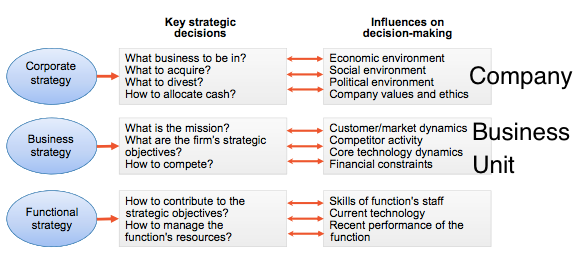
\includegraphics[width=1\textwidth]{W02/strategic_hierarchy}
\subsubsection{Mintzberg's Concept of Emergent Strategy}
\index{Mintzberg's Concept}
\index{Emergent Strategy}
\index{Strategy!Emergent}
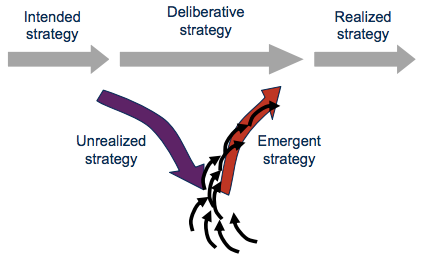
\includegraphics[width=1\textwidth]{W02/mintzberg}
\subsubsection{Good - Cheap - Fast}
Pick two :)
\subsubsection{Tradeoffs - The 'Efficient Frontier' \index{Efficient Frontier} View}
ABCD haben ''Best Practice''\index{Best Practice} erreicht, aus Sicht X ist B der gr\"osste Konkurrent.
B1 zeigt das Best in Class\index{Best in Class} ein nachhaltiger Vorteil ist.\\
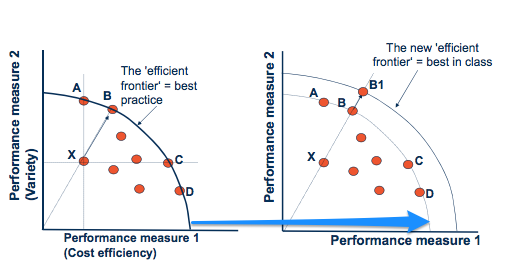
\includegraphics[width=1\textwidth]{W02/efficient_frontier}